\documentclass[a4paper,10pt]{scrartcl}
\usepackage[utf8]{inputenc}
\usepackage[naustrian]{babel}
\usepackage{amsmath}
\usepackage{graphicx}
\usepackage{tabularx}
\usepackage{hyperref}

%opening
\title{Human Computer Interaction und Psychologie - Meilenstein 2}
\subtitle{Elektronisches Curriculum}
\author{Team 1 \\Pascal Attwenger, Philipp Hiermann, Sandra Markhart}

\begin{document}

\maketitle

\section*{Beschreibung der Prototypen}

\subsection*{Low-Fidelity-Prototyp}

\subsubsection*{eCurriculum}

 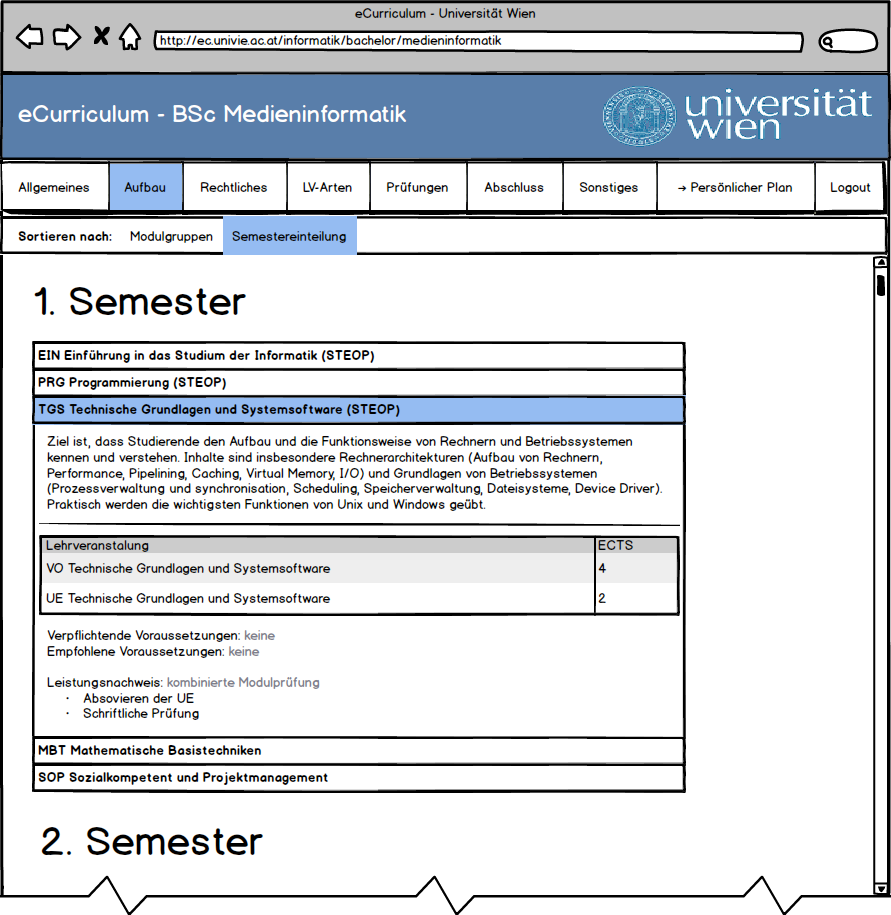
\includegraphics[scale=0.4]{./lowfi-curriculum.png}\\
 
Das eCurriculum soll für Studierende als Ersatz für das derzeitige Mitteilungsblatt dienen. Die Vielzahl an Paragraphen soll thematisch auf mehrere Seiten aufgeteilt werden, damit die benötigten Informationen schneller gefunden werden können und nicht erst mühsam in einem langen, unübersichtlichen Dokument gesucht werden müssen.

Das Hauptaugenmerk der Curriculums soll in der übersichtlichen Präsentation des Studienaufbaus liegen. Hierbei soll möglich sein, die verschiedenen Module auf mehrere Arten zu sortieren. Insbesondere sollte die Sortierung nach Modulgruppen sowie nach der empfohlenen Semestereinteilung möglich sein.

Bei einem Klick auf ein Modul soll sich ein Infobereich mit den wichtigsten Eigenschaften des Moduls öffnen: Beschreibung, ECTS-Aufteilung, Voraussetzungen etc. Um die Menge der gleichzeitig angezeigten Informationen in Grenzen zu halten, sollte sich der Bereich wieder schließen, wenn ein neuer Bereich geöffnet wird; es ist also eine Implementierung als Accordion angedacht.

\subsubsection*{Persönlicher Plan}

Neben den allgemeinen Informationen, die für alle Studierenden eines Fachs die gleichen sind, soll das eCurriculum in Form eines persönlichen Plans auf übersichtliche Weise den individuellen Studienfortschritt aller Studierenden darstellen; damit ersetzt es die Rubriken \emph{Leistungsübersicht} bzw. \emph{Prüfungspass} im aktuellen Univis-System.\\

 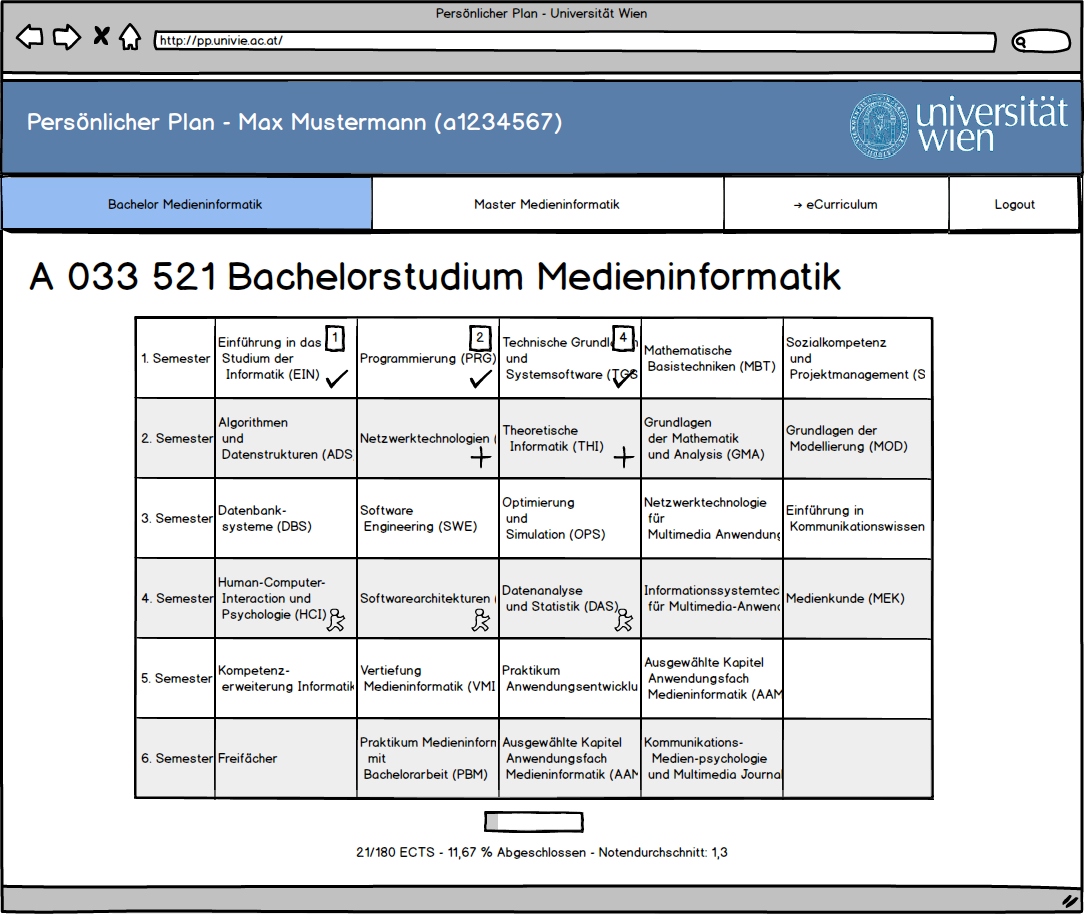
\includegraphics[scale=0.35]{./lowfi-plan.png}\\

Als Übersichtsansicht soll der Musterstudienplan in tabellarischer Form gezeigt werden. Hier werden die essentiellen Informationen auf den ersten Blick präsentiert: Mittels Symbolen und Farbcodierung wird gezeigt, ob ein Modul ganz, teilweise oder noch nicht abgeschlossen wurde; bei abgeschlossenen Modulen wird zudem die berechnete Modulnote gezeigt.

Außerdem soll der Studienfortschritt (auf ECTS-Punkte bezogen) sowie der Notendurchschnitt visualisiert werden. 

\subsubsection*{Modulansicht}

 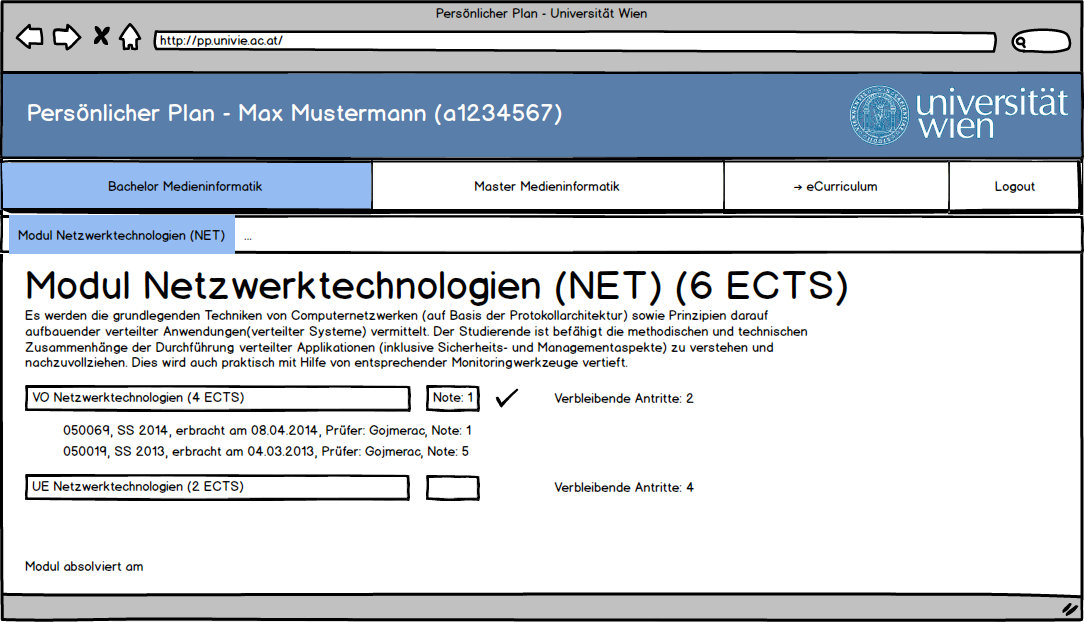
\includegraphics[scale=0.35]{./lowfi-modul.png}\\

Bei einem Klick auf ein Modul im Plan öffnet sich die Detailansicht des Moduls. Hier findet sich neben der Kurzbeschreibung des Moduls die Aufspaltung in alle zugehörigen Lehrveranstaltungen. Alle erbrachten Leitungen werden mit Note und Datum angezeigt, ebenso wie die Anzahl der noch verbleibenden Antritte.

Wurde das Modul ganz abgeschlossen, so findet sich auch hier die Modulnote mit zugehörigem Datum.

\newpage
\subsection*{High-Fidelity-Prototyp}

\begin{description}
 \item[Url:] \url{http://wwwlab.cs.univie.ac.at/~a1151917/hci/}
 \item[Datei auf cewebs:]Meilenstein 2 - Team 1 - Webseite
  \begin{itemize}
  \item css/: CSS-Dateien von Bootstrap und eine angepasste CSS-Datei ``ecurriculum.css''
  \item js/: Java-Script-Dateien von Bootstrap
  \item fonts/: Fonts und Glyphicons von Bootstrap
  \item plan/: PHP-Dateien zum persönlichem Plan, der Überprüfung der aktuellen Session, Login/Logout und eine modifizierte csv-Datei
  \item ecurriculum/: PHP-Dateien zum eCurriculum
  \item img/: Logo der Universität Wien
 \end{itemize}
\end{description}

\begin{description}
 \item[Login-Daten:] 
 \begin{itemize}
  \item[]
  \item Matrikelnummer: a1234567
  \item Passwort: passwort
 \end{itemize}

\end{description}

\subsubsection*{Startseite}

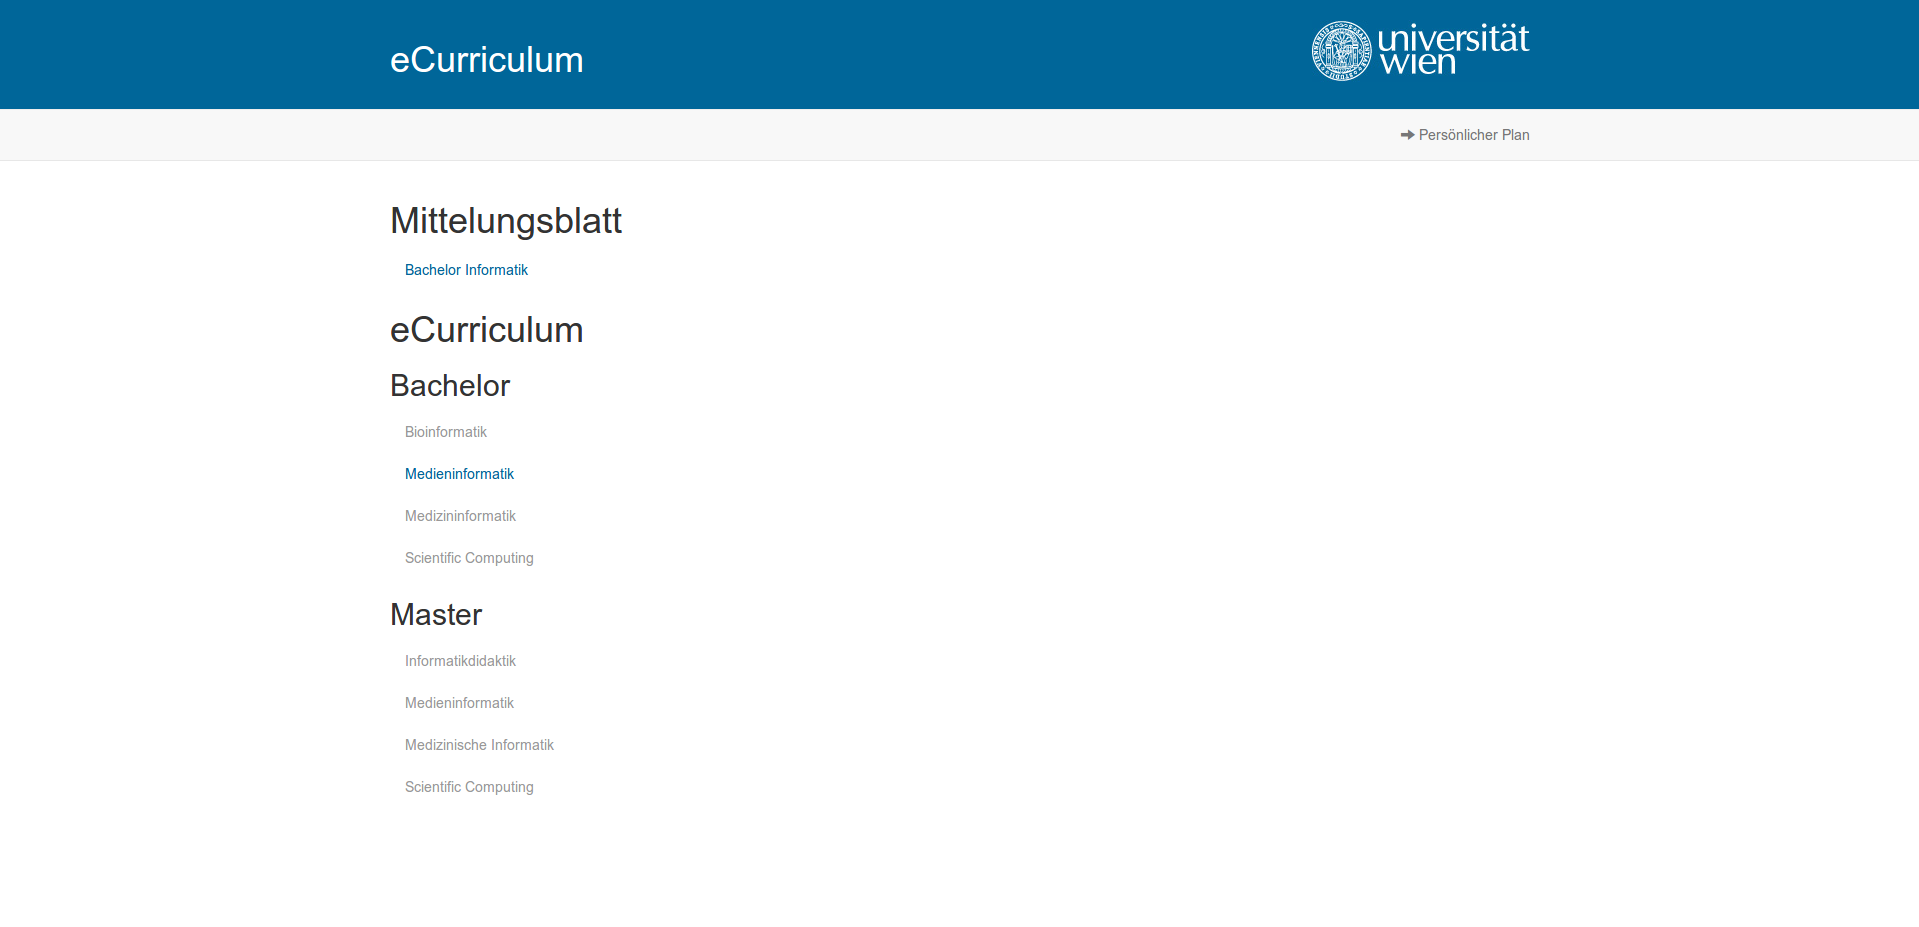
\includegraphics[scale=0.19]{./hifi_screenshots/hifi_startseite.png}\\

Von hier aus gelangt man zu allen möglichen Menüpunkten. Die Startseite ist jederzeit durch Klicken auf das Emblem der Universität am rechten oberen Rand zu erreichen. Für jedes Studium gibt es die gleichen Menüunterpunkte.

\subsubsection*{Allgemeines}


\includegraphics[scale=0.19]{./hifi_screenshots/hifi_allgemeines.png}\\

Hier bekommt man allgemeine Informationen über das Studium.

\subsubsection*{Aufbau}

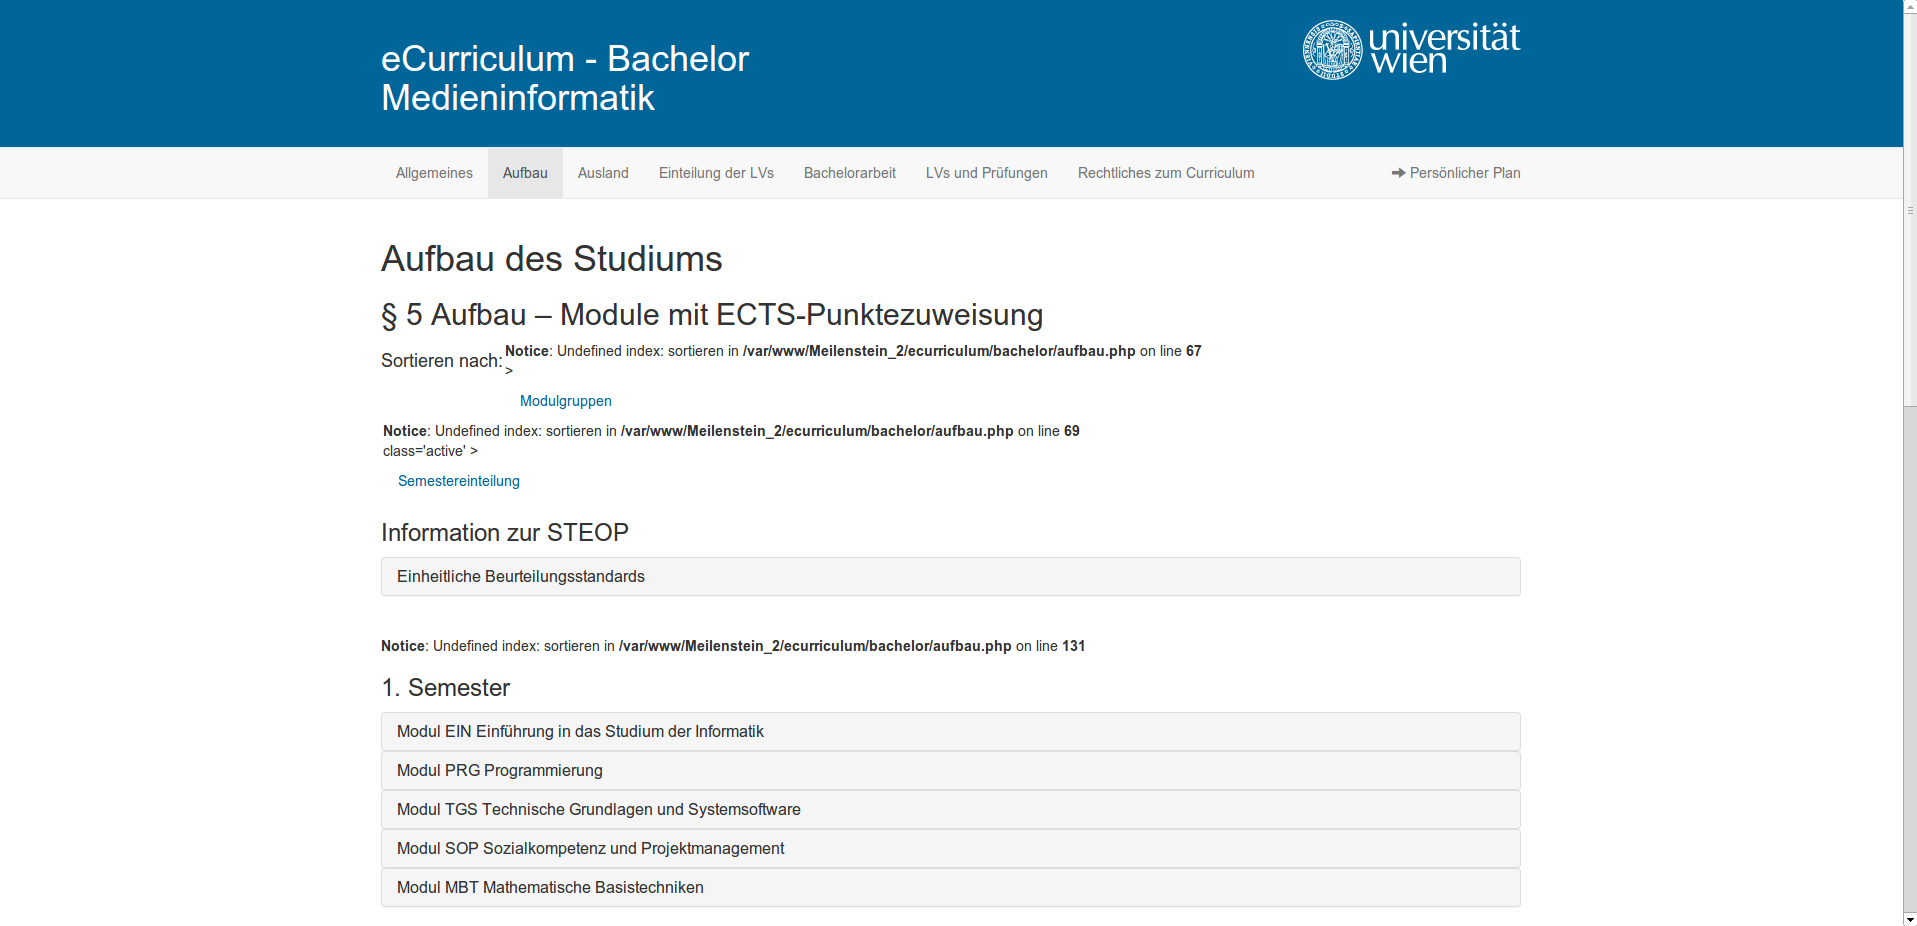
\includegraphics[scale=0.19]{./hifi_screenshots/hifi_aufbau1.png}\\

Hier sieht man alle Module, die absolviert werden müssen.

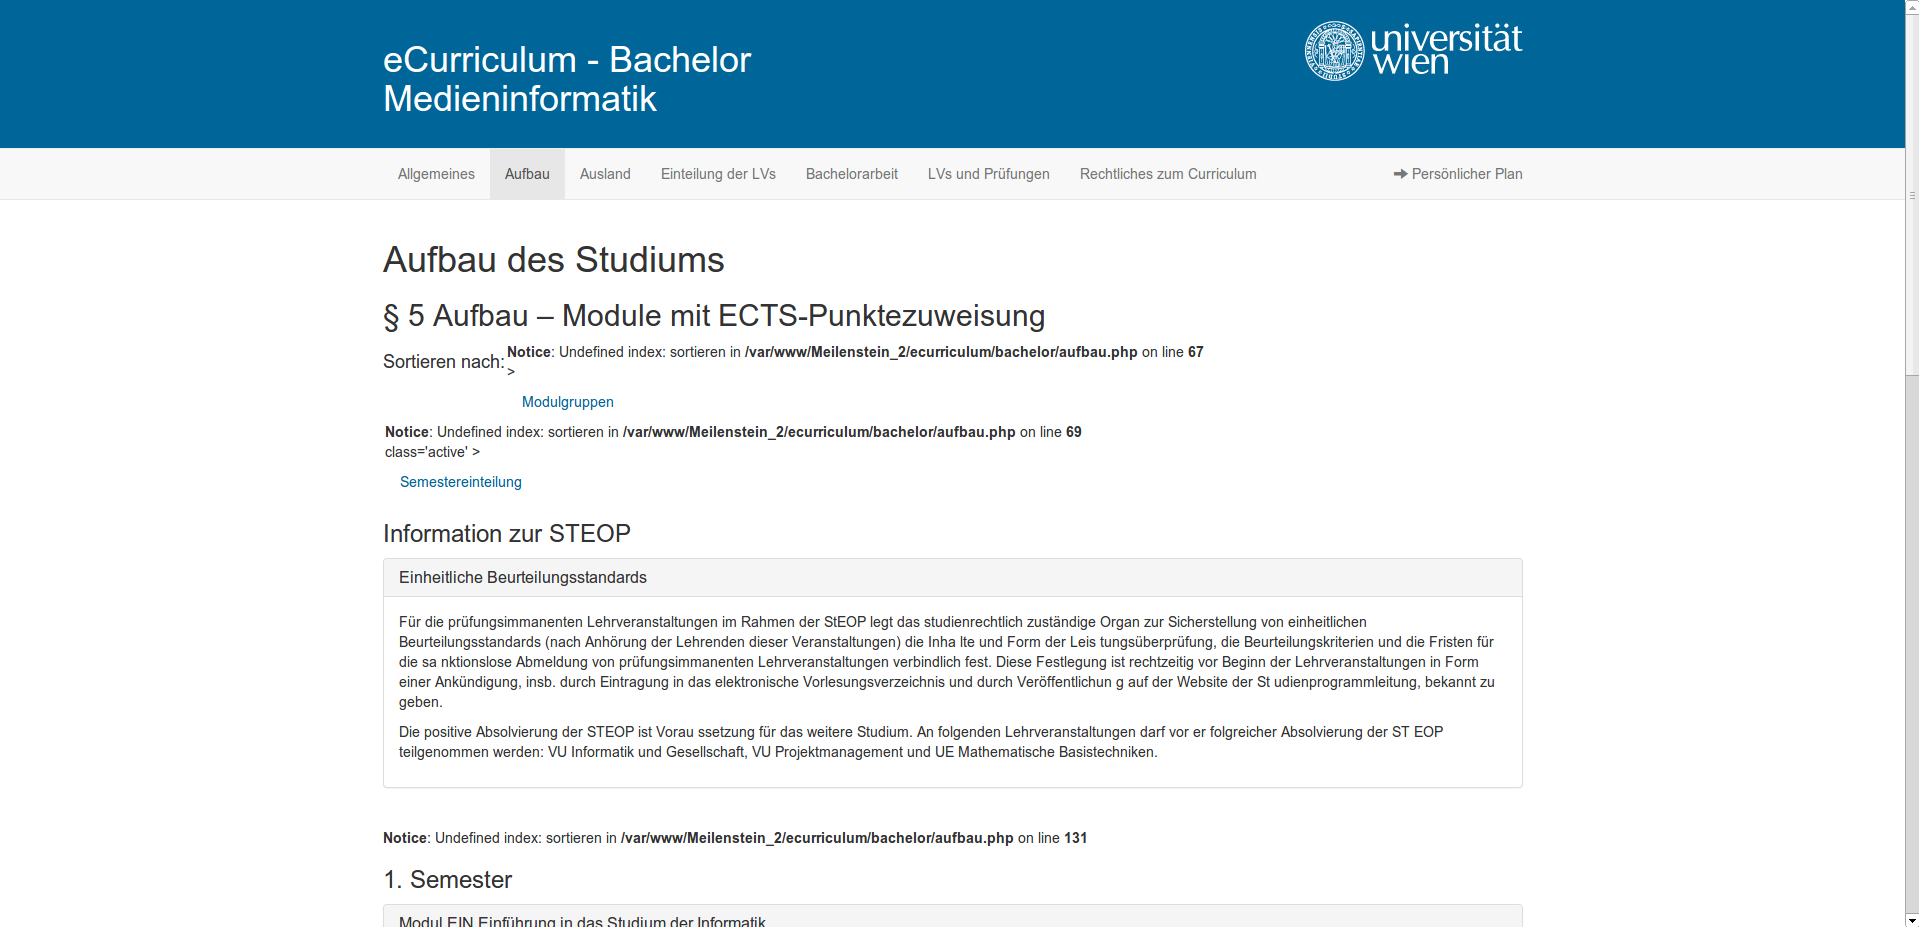
\includegraphics[scale=0.19]{./hifi_screenshots/hifi_aufbau2.png}\\

Für detailliertere Information können die einzelnen Menüs aufgeklappt werden.

\subsubsection*{Ausland}


\includegraphics[scale=0.19]{./hifi_screenshots/hifi_ausland.png}\\

Unter dieser Rubrik sind Informationen zu Auslandssemestern verfügbar.

\subsubsection*{Einteilung}


\includegraphics[scale=0.19]{./hifi_screenshots/hifi_einteilung.png}\\

Hier sollen die Nutzer einen Überblick darüber bekommen, welche Arten von Lehrveranstaltungen es gibt.

\subsubsection*{Bachelorarbeit}

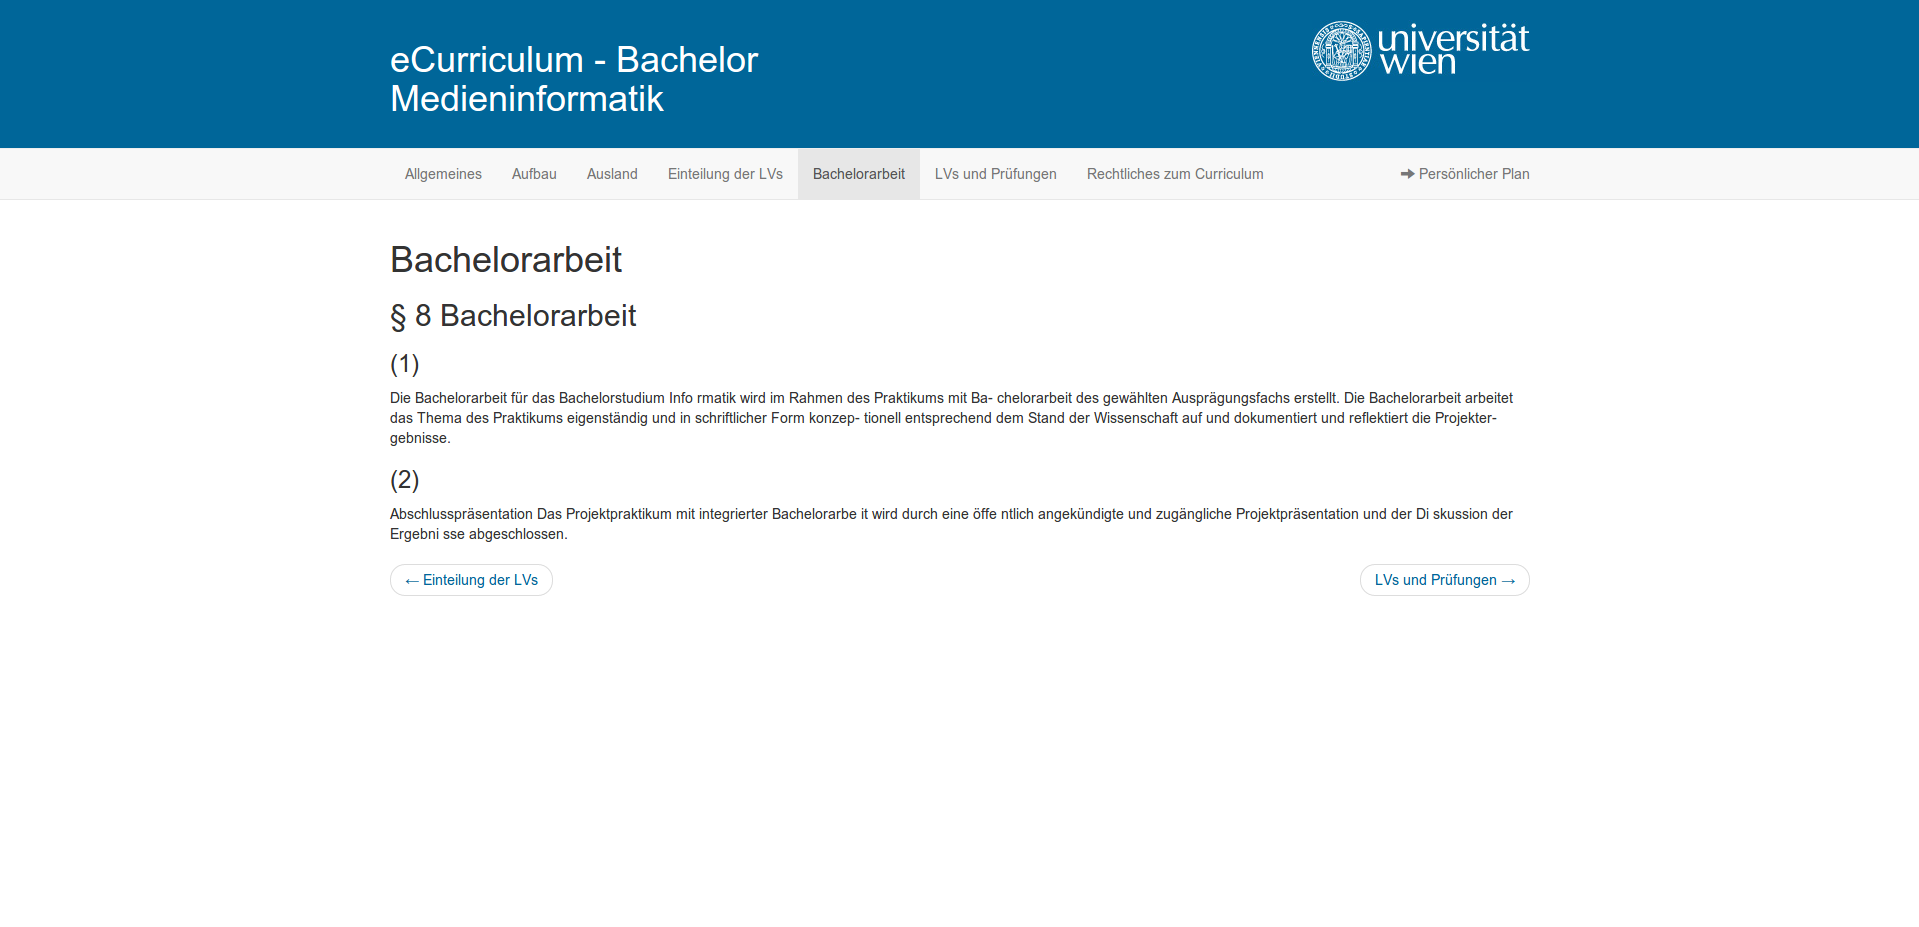
\includegraphics[scale=0.19]{./hifi_screenshots/hifi_bachelor.png}\\

Hier werden die rechtlichen Grundlagen, die für die Bachelorarbeit gelten angezeigt.

\subsubsection*{LV und Prüfungen}


\includegraphics[scale=0.19]{./hifi_screenshots/hifi_lv.png}\\

Hier können rechtliche Informationen zu Lehrveranstaltungen und Prüfungen eingesehen werden.

\subsubsection*{Rechtliches}


\includegraphics[scale=0.19]{./hifi_screenshots/hifi_recht.png}\\

Sonstige rechtliche Informationen.

\subsubsection*{Login}

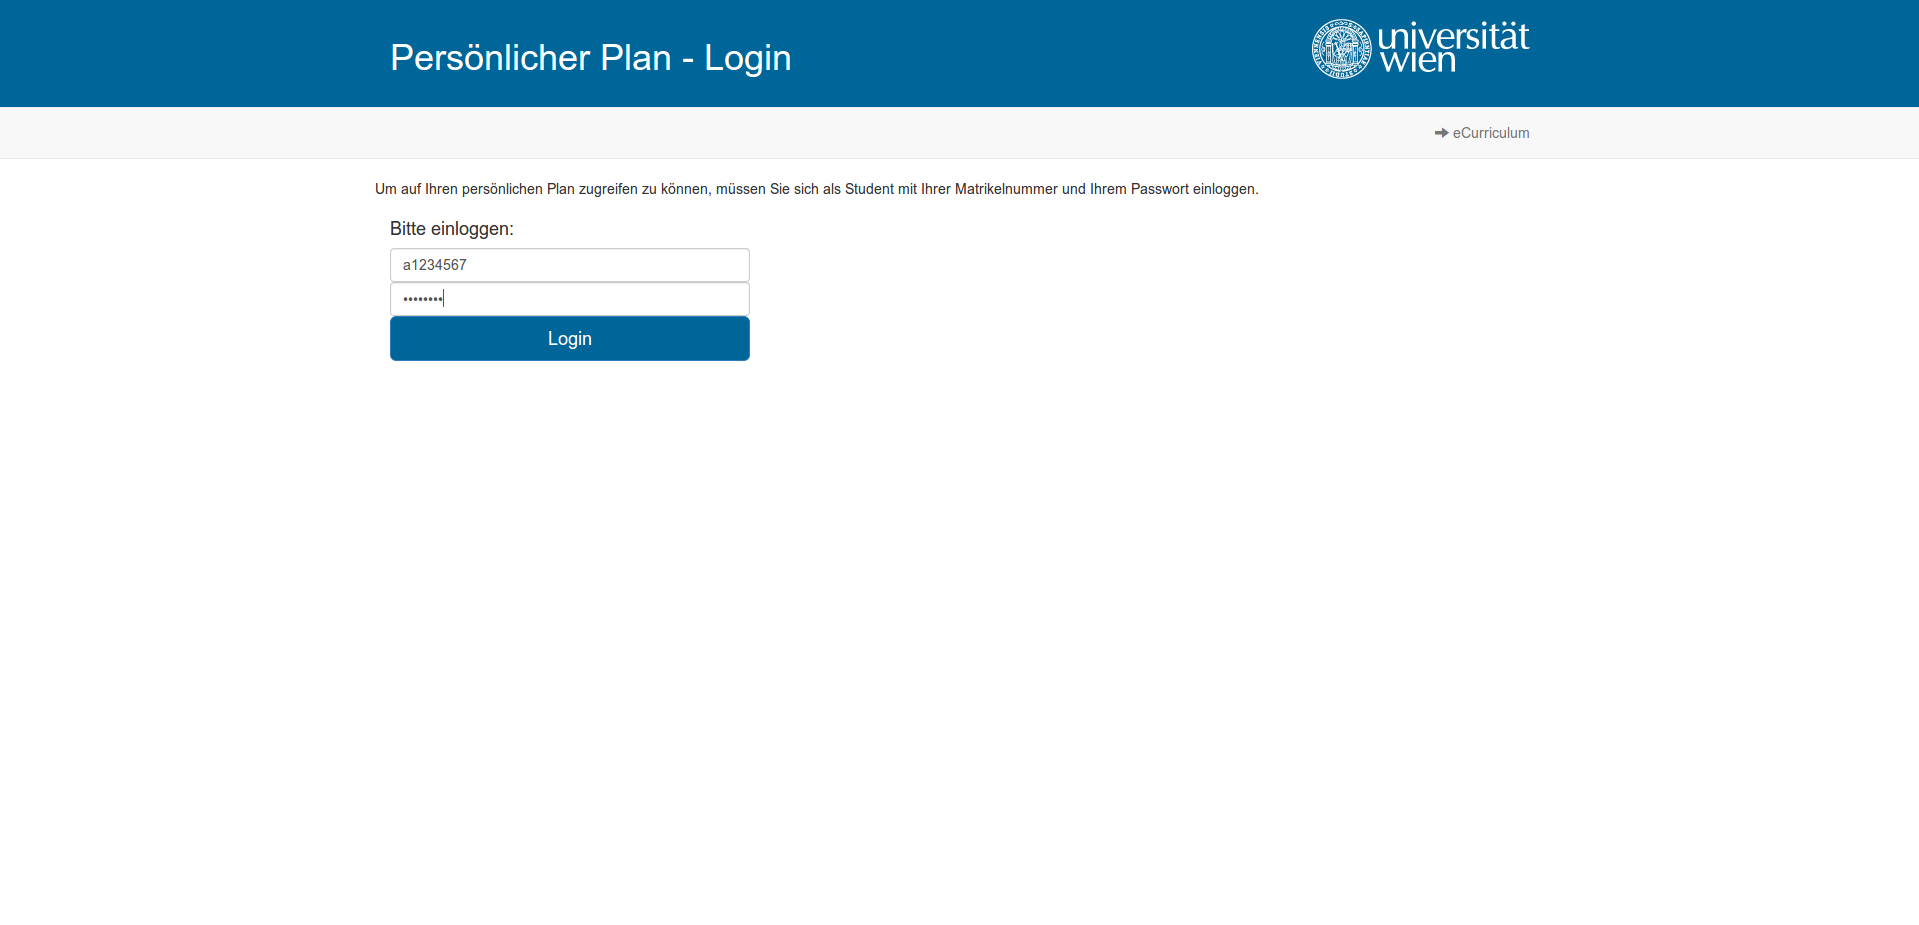
\includegraphics[scale=0.19]{./hifi_screenshots/hifi_login.png}\\

Eine simple Login-Maske

\subsubsection*{Persönlicher Plan}

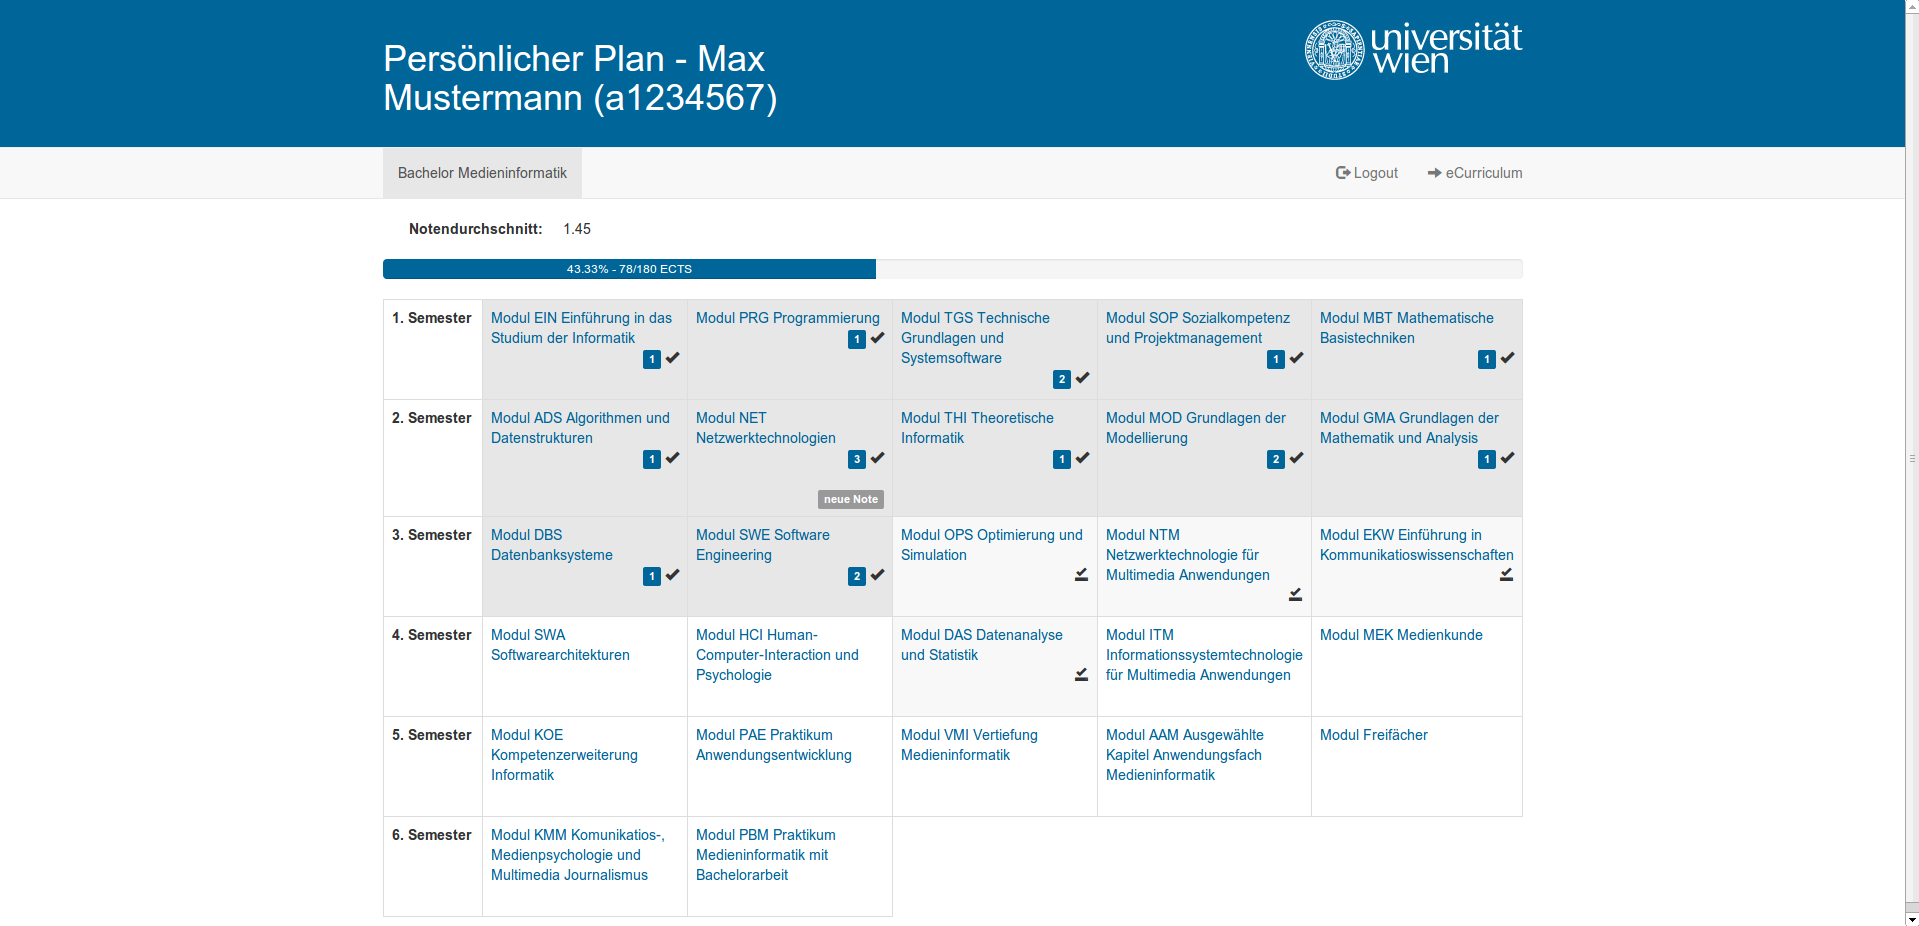
\includegraphics[scale=0.19]{./hifi_screenshots/hifi_persplan.png}\\

Hier kann man seinen persönlichen Fortschritt betrachten. Zu jedem Modul ist sofort ersichtlich, ob es schon absolviert wurde oder nicht.

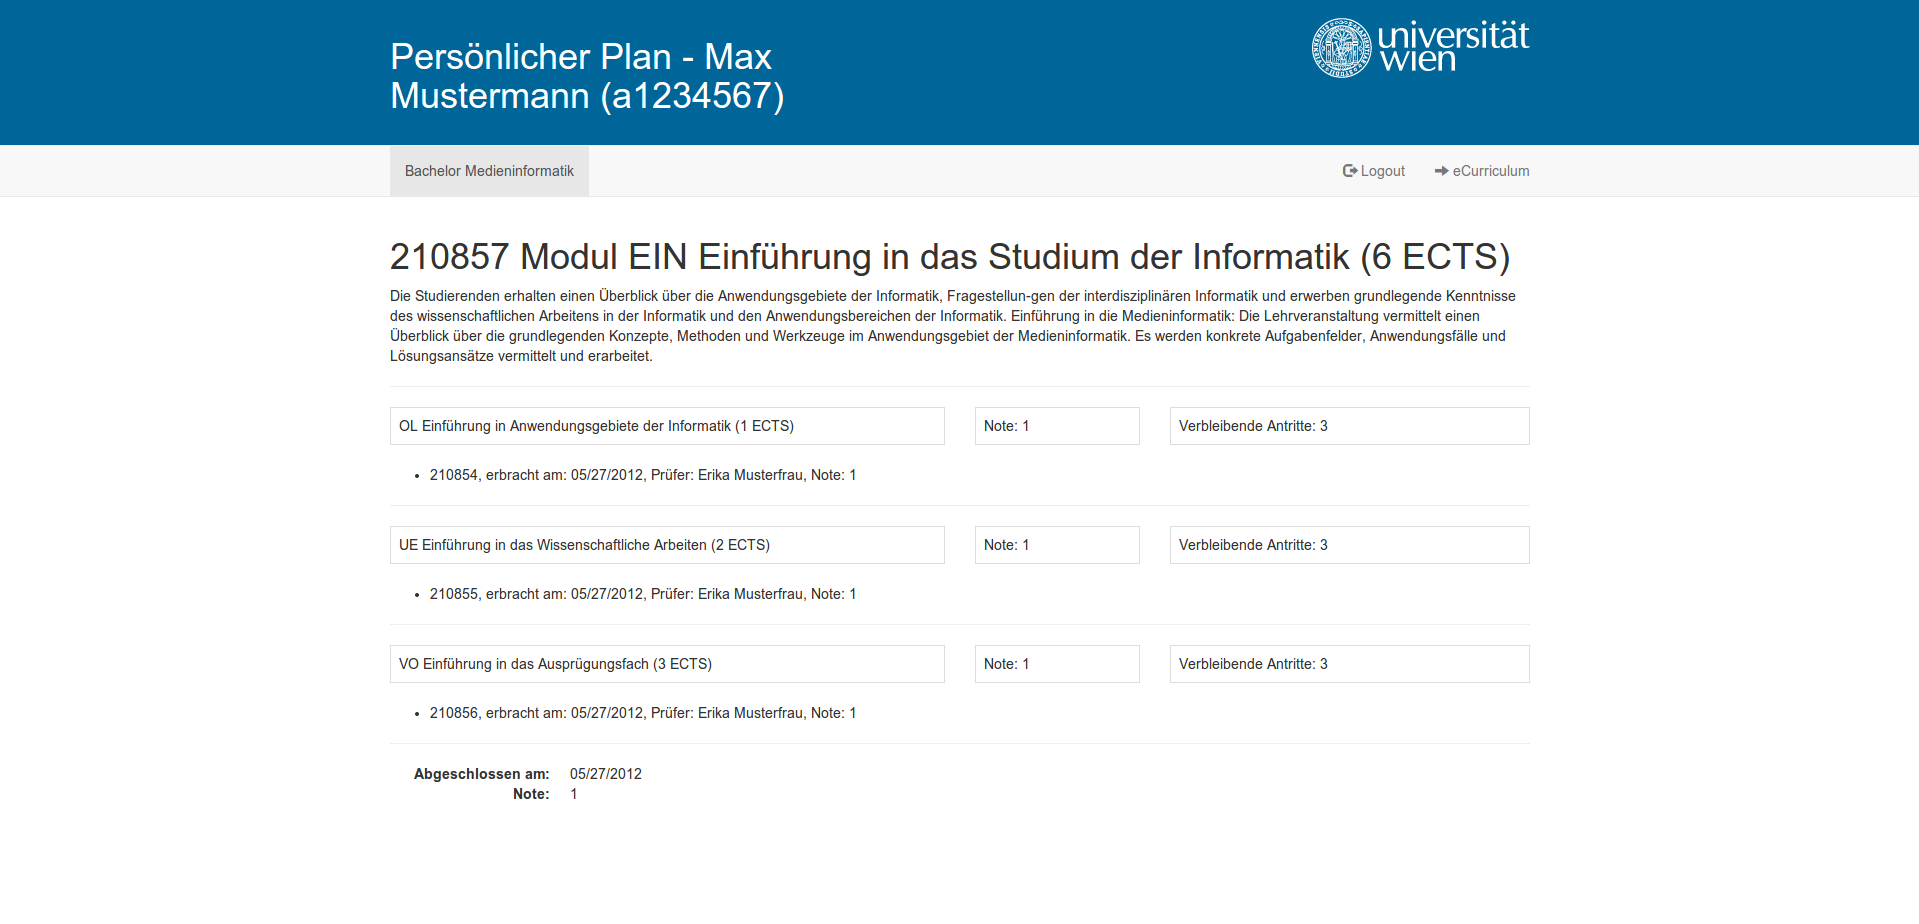
\includegraphics[scale=0.19]{./hifi_screenshots/hifi_persplan2.png}\\

Wie auch schon beim Menüpunkt Aufbau ist es auch möglich, mehr Informationen (wie zB die Einzelnoten) durch Aufklappen der einzelnen Module zu erhalten.

\section*{Interview}

\subsection*{Vorgehensweise}

\subsection*{Ergebnisse}

\section*{Begründen der Designentscheidungen}
Das System richtet sich in erster Linie an Studierende; hierbei werden zwei Nutzungstypen unterschieden: Einerseits sollen Studienanfänger leicht an die für sie nötigen Informationen gelangen können, andererseits sollen fortgeschrittene Studierende einfach und übersichtlich ihren derzeitigen Studienfortschritt einsehen können.

In der Implementierung wurde dies durch eine Zweiteilung des Systems erreicht: Das eCurriculum, das die Mitteilungsblätter in allen praktischen Belangen ersetzen soll, ist – genau wie diese – öffentlich einsehbar. Die (rechtlichen) Informationen wurden auf mehrere Unterseiten aufgeteilt und sind so weniger überwältigend und intuitiver auffindbar.

Beim Studienablauf ermöglicht die nach empfohlener Semesterzuordnung sortierte Ansicht eine schnelle Erfassung der Modulabfolgen; darauf basierend lässt sich die Semesterplanung besser vornehmen, als das beim alten Mitteilungsblatt der Fall war. Besonders für Erstsemestrige stellt dies eine erhebliche Verbesserung dar.

Eine Designentscheidung, die aus Gründen der Übersichtlichkeit getroffen wurde, war, den beispielhaften BSc-Studienplan der Informatik mit seinen 4 Ausprägungsfächern auf 4 einzelne Studienpläne aufzuteilen; bei der tatsächlichen Anwendung in der Praxis müsste geprüft werden, ob diese Abstraktion mit den gegebenen rechtlichen Umständen vereinbar wäre.

Der zweite Teil des Systems, der persönliche Semesterplan, richtet sich gezielt an Studierende, die ihr Studium bereits begonnen haben, und ist daher durch eine Anmeldemaske mit den u:net-Daten zugriffsbeschränkt.

(Für den Prototypen wurde die Anmeldung mit Beispieldaten selbst implementiert. In der tatsächlichen Anwendung wäre dies natürlich in das bestehende Anmeldesystem eingebunden.)

Als Designentscheidungen ist hierbei zu erwähnen, dass die Markierung der Module – hinsichtlich ``abgeschlossen", ``teilweise abgeschlossen" oder ``noch nicht abgeschlossen" – nicht wie bisher in schriftlicher Form passiert, sondern sowohl durch Farbmarkierung wie auch durch Symbole. Farblich wurde nicht wie ursprünglich angedacht ein Ampelsystem verwendet, sondern eine Abstufung dreier Grautöne. Einerseits, weil es sich so rein ästhetisch besser in das Farbkonzept einbindet, aber auch um Diskriminierung bezüglich Farbenfehlsichtigkeit vorzubeugen.

Zuletzt wurde auch eine optische Markierung – ``Neue Note" – eingeführt, um Verän-derungen seit dem letzten Login schnell sichtbar zu machen.

\section*{Typische Fehlermeldungen}

\subsubsection*{Aufrufen des persönlichen Plans ohne eingeloggt zu sein}

Eine typische Fehlermeldung ist, wenn der Benutzer den persönlichen Plan aufrufen will und sich noch nicht zuvor mit seinen Benutzerdaten eingeloggt hat,
da der persönliche Plan nur Studierenden zugänglich ist. Der Benutzer wird dann darauf hingewiesen, dass er sich einloggen muss.

\begin{quote}
 \textit{``Um auf Ihren persönlichen Plan zugreifen zu können, müssen Sie sich als Student mit Ihrer Matrikelnummer und Ihrem Passwort einloggen.''}
\end{quote} 

\begin{center}
 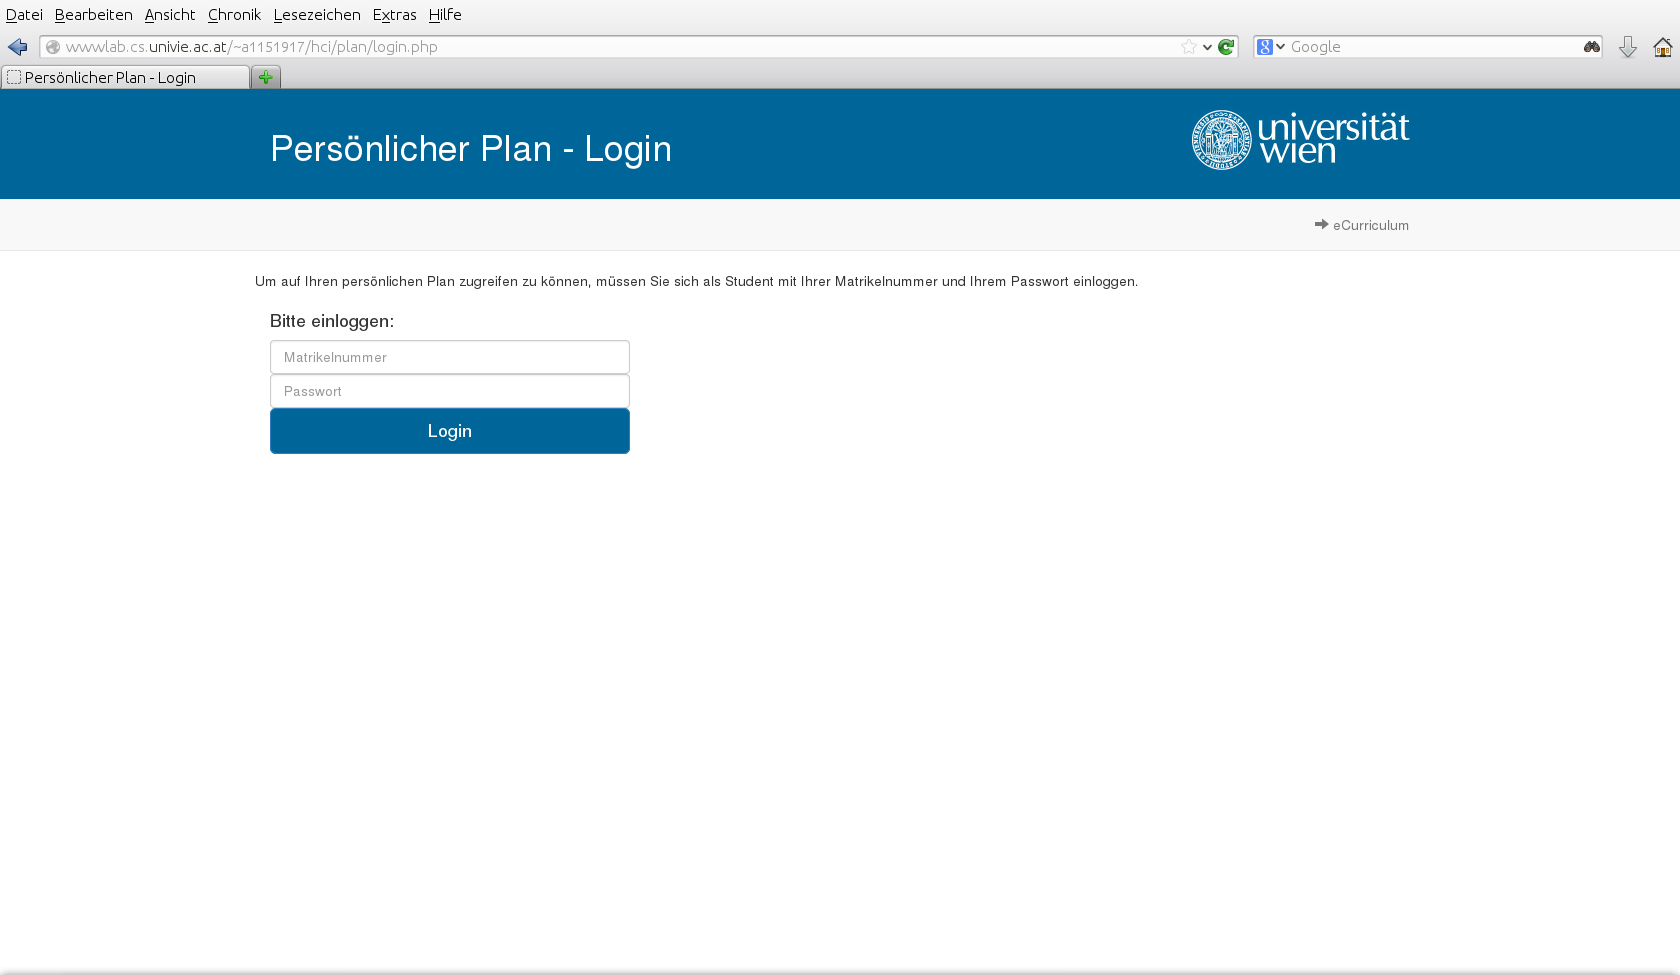
\includegraphics[scale=0.4]{./fehlermeldung1.png}
 % fehlermeldung1.png: 1680x975 pixel, 120dpi, 35.56x20.64 cm, bb=0 0 1008 585
\end{center}


\subsubsection*{Login mit falschem Benutzernamen oder falschem Passwort}

Eine weitere typische Fehlermeldung erscheint, wenn der Benutzer sich versucht einzuloggen, aber einen falschen Benutzernamen oder ein falsches Passwort eingibt.
Dieser wird dann je nachdem auf das falsche Passwort oder den falschen Benutzernamen hingewiesen.

\begin{quote}
 \textit{``Diese Matrikelnummer existiert nicht.''}
\end{quote} 

\begin{center}
 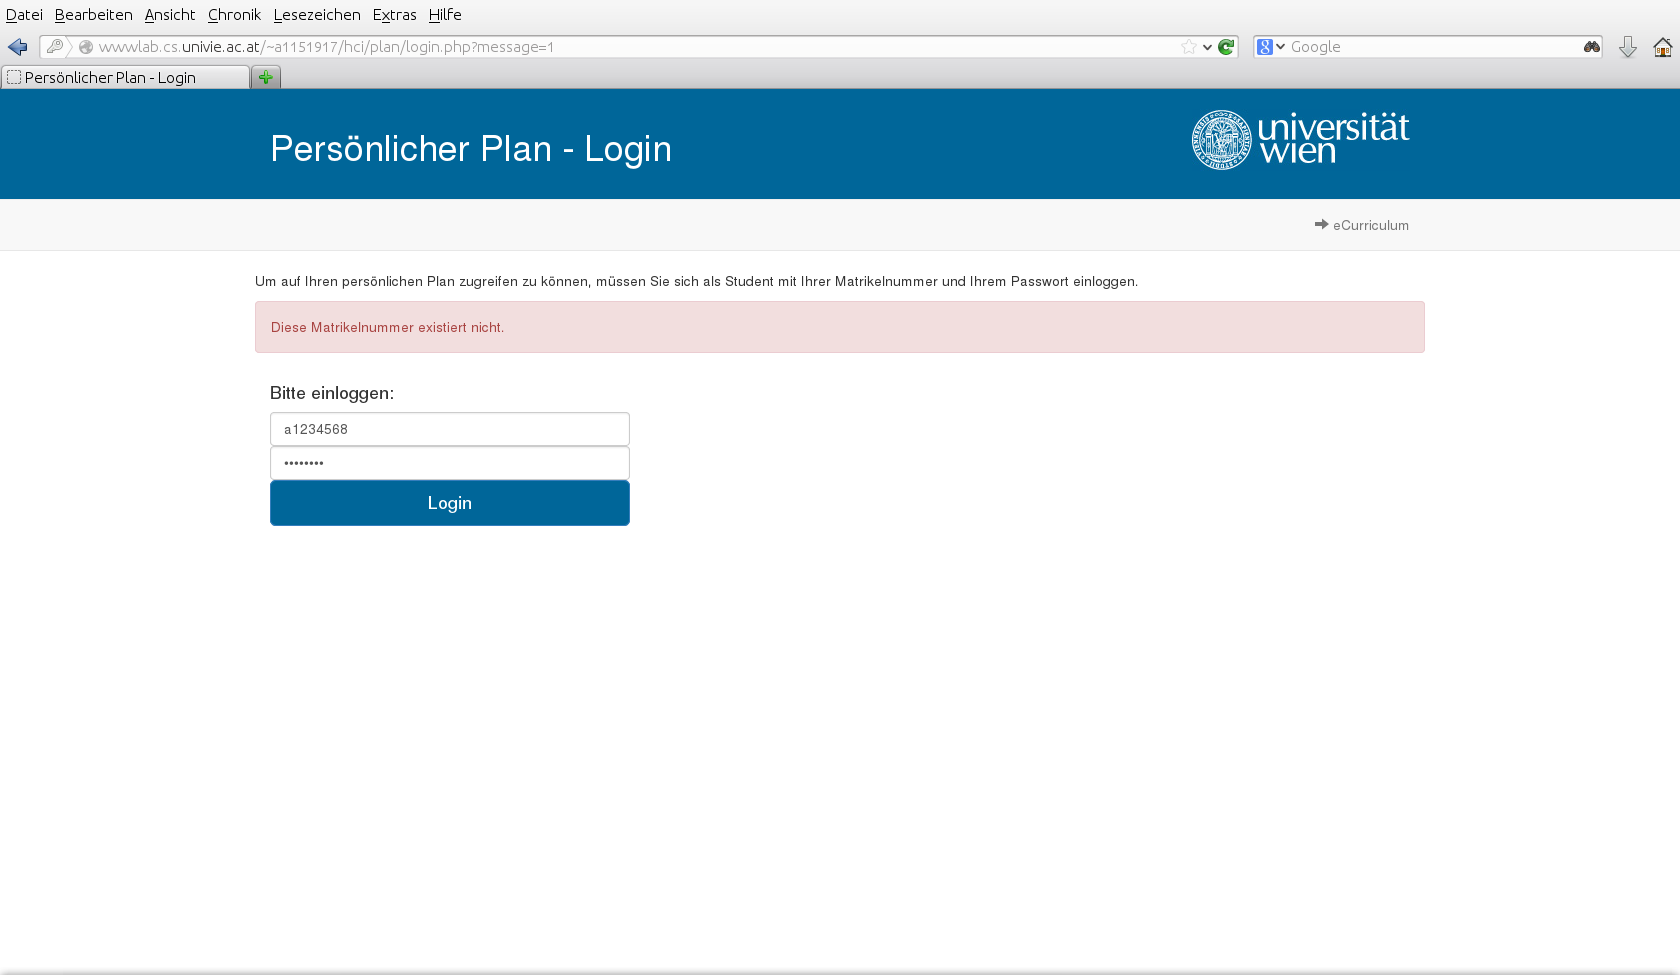
\includegraphics[scale=0.4]{./fehlermeldung2.png}
 % fehlermeldung1.png: 1680x975 pixel, 120dpi, 35.56x20.64 cm, bb=0 0 1008 585
\end{center}

Zusätzlich könnte zu der Fehlermeldung, dass die Matrikelnummer falsch ist dann noch die eingegebene Matrikelnummer angezeigt werden und gegebenenfalls darauf hingewiesen
werden, dass diese aus a + 7 Ziffern bestehen muss.

\begin{quote}
 \textit{``Das Passwort ist falsch.''}
\end{quote} 

\begin{center}
 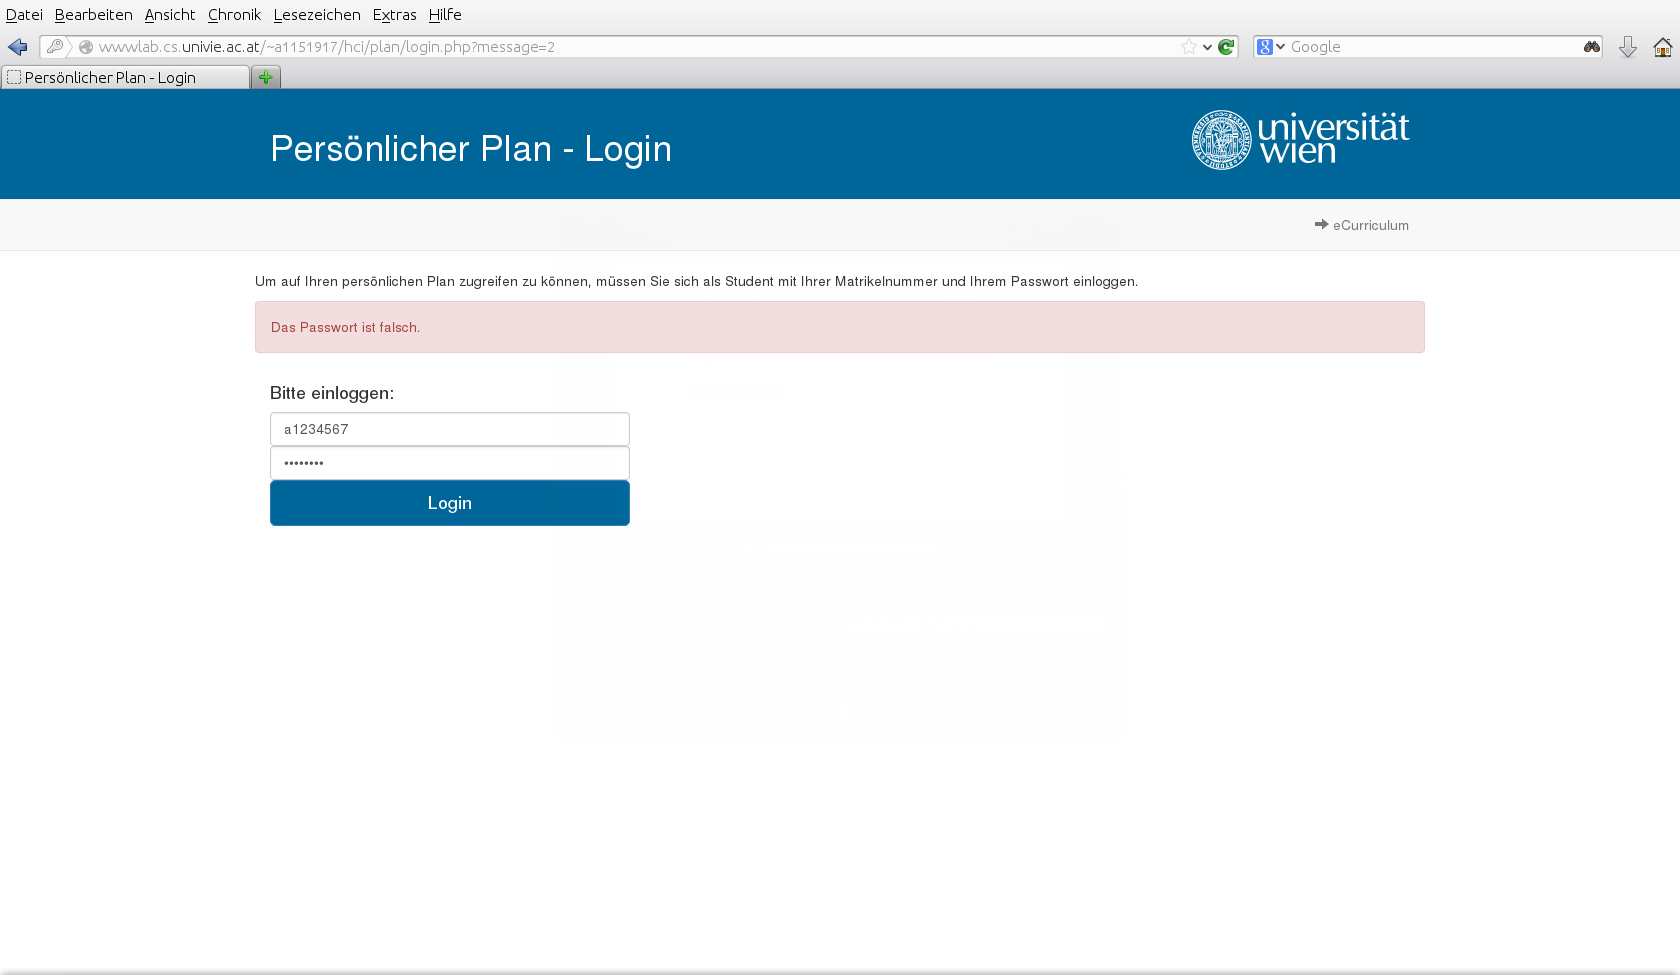
\includegraphics[scale=0.4]{./fehlermeldung3.png}
 % fehlermeldung1.png: 1680x975 pixel, 120dpi, 35.56x20.64 cm, bb=0 0 1008 585
\end{center}

Hier könnte zusätzlich entweder noch eine ``Passwort vergessen''-Funktion eingebaut werden, welche es ermöglicht das Passwort selbst zurückzusetzen oder einen
Hinweis auf z.B. den ZID gegeben werden, welcher in solchen Situationen weiterhilft.

\subsubsection*{Aufrufen eines nicht vorhandenen Moduls}

Auch könnte eine typische Fehlermeldung erscheinen, wenn eine Seite aufgerufen wird, welche nicht existiert. Dies kann hier auftreten wenn ein Modul aufgerufen wird, indem die Modulid in der Adressleiste
eingegeben wird, zu der kein Modul existiert.

\begin{quote}
 \textit{``Das Modul mit der Modulnummer 210324 existiert nicht.''}
\end{quote} 

\begin{center}
 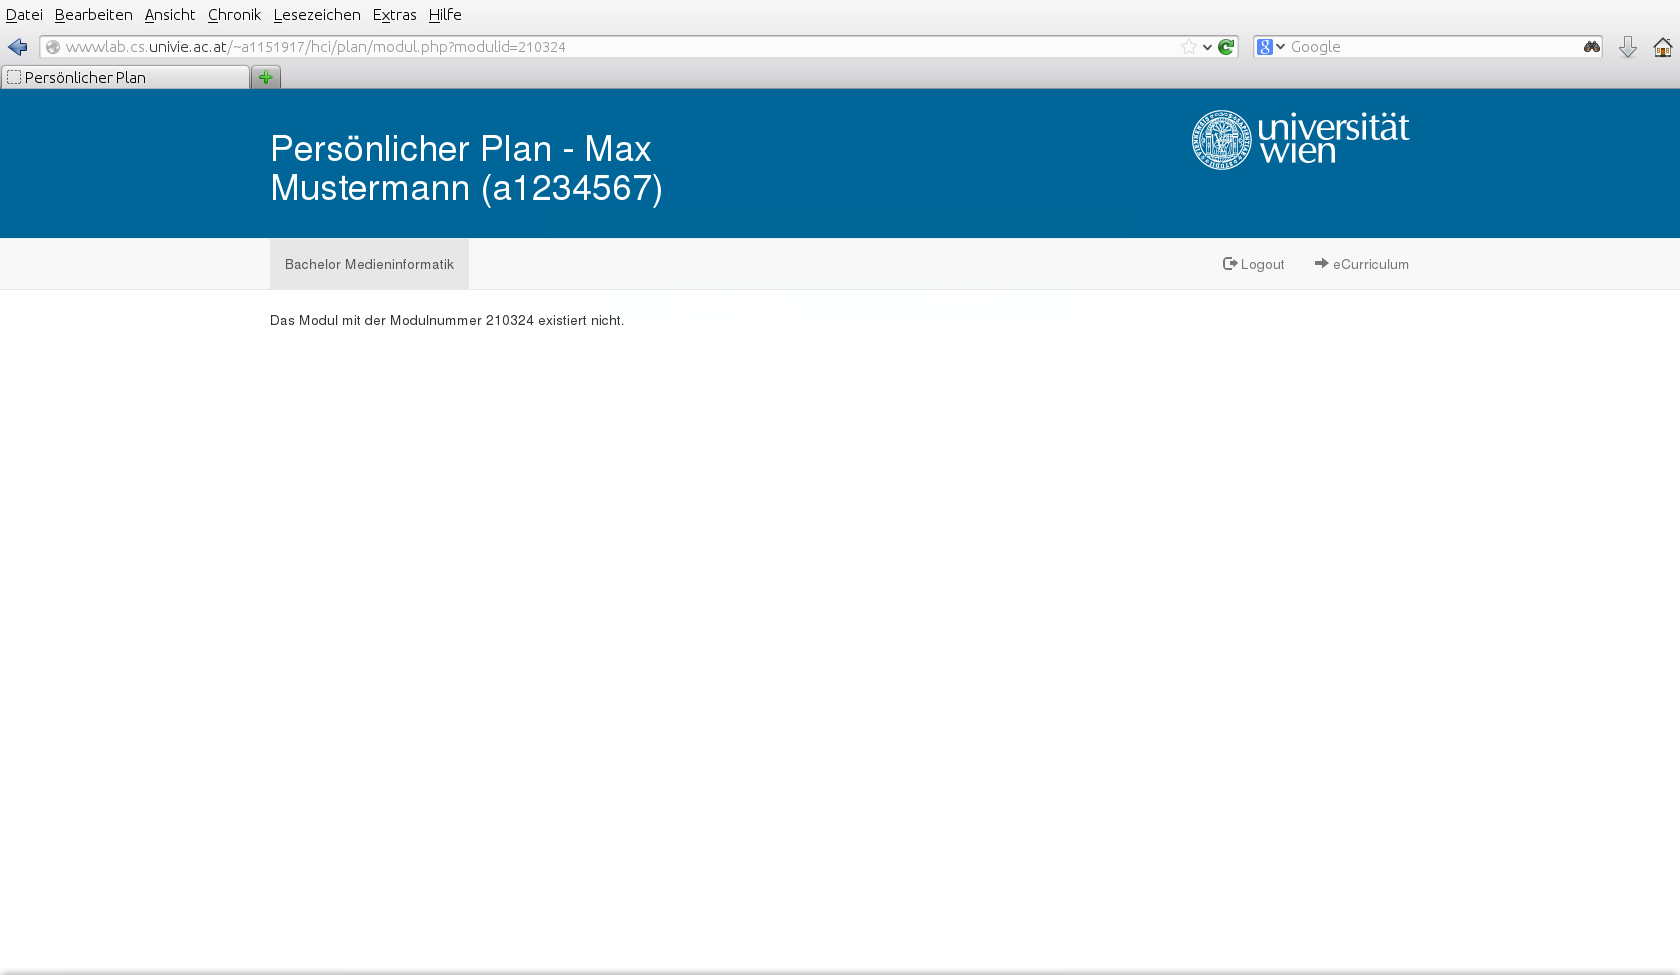
\includegraphics[scale=0.4]{./fehlermeldung4.png}
 % fehlermeldung1.png: 1680x975 pixel, 120dpi, 35.56x20.64 cm, bb=0 0 1008 585
\end{center}



\end{document}



